
\documentclass[a4paper]{article}
\usepackage[T1]{fontenc}
\usepackage[english]{babel}
\usepackage[utf8]{inputenc}
\input Sanremo.fd
\usepackage[
  top=0.5cm,
  bottom=0.5cm,
  left=1cm,
  right=1cm,
  headheight=17pt, % as per the warning by fancyhdr
  includehead,includefoot,
  heightrounded, % to avoid spurious underfull messages
]{geometry} 

\usepackage{tikz}
\usepackage{titlesec}
\usepackage{multicol}
\usepackage{caption}
\newenvironment{Figure}
  {\par\medskip\noindent\minipage{\linewidth}}
  {\endminipage\par\medskip}
\usepackage{fontawesome}
\newcommand{\LeClub}{{\fontsize{10pt}{10pt}\usefont{U}{Sanremo}{xl}{n}Le\hspace{2pt}Club}}
\usepackage{fancyhdr}
\pagestyle{fancy}
\fancyhead[R]{}
\fancyhead[L]{}
\renewcommand{\headrulewidth}{0pt}
\fancyfoot[R]{Version 1.0.0}
\usepackage{soul}

\begin{document}
\begin{multicols*}{2}[
\begin{center}
{\fontsize{72pt}{80pt}\usefont{U}{Sanremo}{xl}{n}Le Club}
\end{center}
]

Det er torsdag aften. Natten er ung og dig og dine venner har kun et mål for øje... \LeClub s VIP-lounge! Men det er ikke hvem som helst der bliver lukket derop. I skal alle samle nok fame på klubben før i kan fejre jeres bedrift i den ypperste luksus. På vejen skal i passe på både fristelser, dørmænd og selvfølgelig de andre gæster på klubben, der kun tænker det samme som jer: Vi skal i den VIP-lounge!
\section{Spillerens hold}
\LeClub\ kan spilles hver person for sig selv eller i hold. Spilles der i hold kan tåre og andre holdrelaterede konsekvenser fordeles frit mellem holdets deltagere. Dog må holdet ikke drikke af den samme genstand.

Hver spiller/hold har tre karakterer: To piger og en dreng. Der gælder samme regler for alle karaktererne på nær, at indgang for piger koster 1 pant og indgang for drenge koster 2 pant.
\section{Betalingssystem}

Møntfoden på \LeClub\ er pant. Hver drukket genstand svarer til 1 pant. Ægte spillere af \LeClub\ drikker self kun breezers, men øl går også an.

Det er kun tilladt at have én åben drik af gangen. I holdspil må spillere have hver deres drik, men under spillet må de åbne drikke ikke byttes internt mellem spillerne. Åbnes en ny drik inden den forrige er tømt, skal én af drikkene tømmes før holdet må slå med terningen igen. Indtil da springes holdets tur over. 
\section{Spillets start}
Hvert hold placerer én af deres karakterer på feltet foran \LeClub . Alle andre karakterer starter uden for klubben på det bagerste felt. Alle knapper en frisk breezer op. Den yngste spiller starter. 

For at rykke en karakter, der står uden for klubben skal der slås 5 eller 6 med terningen. Uden for klubben rykkes der ét felt ad gangen. For at rykke en karakter ind fra det sidste felt af fortovet til det første felt på klubben, markeret med en blå stjerne, skal der betales entre. Karakteren, der er betalt entre for, får et stempel og rykkes ind på klubbens første felt efter der er betalt. Stemplet giver adgang til klubben resten af spillet. Entre betales før terningekast. Har et hold ikke en karakter på klubben får man tre forsøg til at slå enten 5 eller 6 med terningen.

En karakter på klubben rykkes det antal felter øjnene på terningen viser. Karakteren kan flyttes både frem og tilbage, men ikke begge dele på samme tur. Ved forgrening rykkes karakteren valgfrit ad en af vejene. Har et hold mere end én karakter på klubben kan holdet selv vælge hvilken karakter der rykkes. Kun én karakter kan rykkes per tur. Når en karakter er sluppet på et gyldigt felt er holdets tur slut. Turen går efterfølgende i negativ omløbsretning. 

Det er i udgangspunktet ikke muligt for to karakterer at stå på samme felt. Spærrer en karakter for at lande på et felt, rykkes karateren i bevægelse til det efterfølgende felt efter normale regler for at rykke. På toilettet og i bagindgangen kan to karakterer stå på samme felt. Dette har ingen konsekvens. Enderne i bagindgangen og på toilettet virker som fuldt stop og kan stoppe alle karakterer lige gyldigt hvor langt karakteren ville rykke videre.
\input{zoner.tex}
\section{Fame}

For at kunne rykke en karakter gennem midten af brættet og op i VIP-loungen skal karakteren have optjent nok fame. I et klassisk spil skal der optjenes 5 fame. Der kan optjenes mere fame end hvad der er nødvendigt.

Fame kan optjenes på flere måder. En karakter kan optjene fame ved chancekortene, der må trækkes når karakteren lander på et rødt felt. En karakter tjener 1 fame for hver ting der købes i baren. En karakter tjener 1 fame ved at blive venner med stripperen eller party-dværgen og tjener 2 fame ved at blive venner med DJ Følerden.

En karakters fame kan ikke være negativ. Vil et tab af fame resultere totalt set i negativ fame bliver karakterens fame i stedet 0.
\section{Dørmanden}
Dørmanden er \LeClub s bouncer! Han er sur og tvær og vil gøre alt for at smide gæster ud. Befinder en karakter sig i samme zone som dørmanden, mens karakteren laver noget man ikke må, får det konsekvenser. Dørmanden starter i bagindgangen og kan ikke rykkes af hold som ikke har en karakter på klubben. Dørmanden rykkes hver gang der slås 1 med terningen. Holdet som har slået 1 rykker en karakter 1 felt og rykker dørmanden til en valgfri zone. Dog kan toilettet, terrassen og garderoben ikke vælges. Efter dørmanden er rykket, går der en runde hvor han er \textit{"på vej"}. Dvs. han ikke kan rykkes af andre hold og at han ikke er aktiv i nogen zone. Dørmanden kan også blive i en zone. I dette tilfælde går der ikke runde før han er på plads. Konsekvenserne ved at blive set af dørmanden (karakteren \textbf{står} i samme zone, når dørmanden er aktiv) er samlet i følgende liste:
\begin{itemize}
\item[$\star$] Ses man med overtøj, sendes man i garderoben.
\item[$\star$] Ses man uden stempel, sendes man ud.
\item[$\star$] Ses man i aggressiv tilstand, sendes man ud.
\item[$\star$] Ses man i bagindgangen, sendes man ud.
\item[$\star$] Ses man med ecstasy, konfiskeres dette
\end{itemize} 

Når man sendes ud af \LeClub\ rykkes karakteren der er sendt ud til det bagerste felt på fortorvet uden for klubben.

Er en karakter venner med dørmanden er vedkommende kun i problemer hvis vedkommende er aggressiv. Resten af forseelserne ses simpelthen bort fra. 
\section{Chancekort}
Nogle af felterne på \LeClub\ er røde. Ender en karakter på et rødt felt må karakterens hold trække et chancekort. Chancekortet læses højt og afvikles før turen gives videre. Alle kort \textbf{skal} afvikles! Kan et hold ikke afvikle kortet udgår holdet af spillet. Efter et kort er afviklet, skal det enten gemmes (fremgår af kortet) eller lægges i bunken med brugte chancekort. Når der ikke er flere chancekort genbruges bunken med brugte kort efter denne er blevet blandet.
\subsection{Telefonnumre}
Trækker en karakter et chancekort med et telefonnummer gemmes kortet indtil opkaldet er udført. Alle karakterer på holdet kan udføre opkaldet, men man kan kun lave opkald på toilettet. Et opkald resulterer altid i venskab mellem karakteren der udfører opkaldet og personen der ringes til. Der ringes før et terningekast, men opkaldet tæller ikke for en tur.
\begin{itemize}
\item[\faPhone] 66 66 66 66 : Dørmanden
\item[\faPhone] 11 22 33 44 : Partydværgen
\item[\faPhone] 12 13 14 15 : Stripperen
\end{itemize}
\subsection{Aggressivitet}
Nogle chancekort gør karakteren der trækker kortet aggressiv. Aggressivitet er et tveægget sværd, der kan være nøglen til at vende eller lukke spillet. For aggressive karakterer gælder der følgende: En aggressiv karakter kan smide en anden karakter ud ved blot at lande på det felt hvor karakteren står. En aggressiv karakter der ses af dørmanden smides straks ud af klubben. Trækker en aggressiv karakter endnu et kort der giver aggressivitet har kortet ingen effekt og det lægges blot i bunken med brugte chancekort. En karakter mister sin aggressivitet hvis karakteren bliver smidt ud eller får et glas vand (se baren).

%\ThisTileWallPaper{\paperwidth}{\paperheight}{rulebook_page.png}

\subsection{Studiekortet}
I blandt chancekortene gemmer det legendariske studiekort sig. Studiekortet giver en karakter dobbelt op på alt i baren. Det er ikke muligt at \textit{give} andre karakterer på sit hold studiekortet. Det er til gengæld muligt at stjæle studiekortet fra karakteren der har det. Dette gøres ved at flytte en karakter over og forbi karakteren med studiekortet. Det er muligt at stjæle studiekortet overalt på \LeClub . Står karakteren med studiekortet på det sidste felt i bagindgangen eller på toilettet er det nok at rykke op på siden af karakteren. Karakteren der får kortet stjålet i dette tilfælde skal først rykke fra feltet for at genstjæle kortet. Når karakteren med studiekortet går op i VIP-loungen udgår studiekortet af spillet. Det lægges \textbf{ikke} i bunken med brugte chancekort.
\subsection{The Golden Ticket}
The Golden Ticket er en alternativ måde at få sine karakterer op i VIP-loungen. Kortet har kun en effekt hvis karakteren der trækker kortet har optjent dobbelt så meget fame som det kræves at komme i VIP-loungen. Har karakteren ikke optjent nok fame lægges kortet blot i bunken med brugte chancekort. Har karakteren optjent nok fame, gemmes kortet ved holdet, indtil det er brugt eller at karakteren smides ud. I dette tilfælde lægges kortet i bunken med brugte chancekort. 

Effekten af The Golden Ticket er spilvindende. Når en karakter med billetten til VIP-loungen med tilstrækkelig fame (\textbf{ikke} dobbelt fame), kan vedkommende tage alle holdets karakterer der er på klubben med op i VIP-loungen, ligegyldigt hvor karaktererne er og hvor meget fame de har optjent. 
\raggedcolumns



\section{Baren}
I baren kan købes forskellige ting, der giver en fordel i spillet. Baren kan benyttes af en karakter der befinder sig på et af de tre grønne felter foran baren. Det tager ikke en tur at bruge baren, men køb skal foretages før terningekast. \textit{Med hvert køb i baren følger 1 fame.} Barens menu kan ses i Tabel \ref{tab}

\begin{Figure}
\centering
\begin{tabular}{p{0.24\textwidth}|p{0.68\textwidth}}
\textbf{Ting \& Pris} & \textbf{Beskrivelse} \\\hline

Partydværg \hspace{0.2cm} 2 pant & Partydværgen (PD) tvinger et hold til at bunde en fuld drik inden holdet må slå med terningen igen. PD må kun bruges på ens egen tur, inden et terningekast. Der kan kun deles én PD ud per tur.\\\hline
%Kongestatus \hspace{2cm}3 pant & En spiller på holdet slikker på bagsiden af et spillekort og placerer kortet i panden \\\hline

Afledningskast $\times 3$ \hspace{2cm} 1 pant & Holdet kan bruge disse til at rykke karakterer gennem bagindgangen (se afledningskast). \\\hline

Afføringspille \hspace{2cm} 2 pant & Holdet kan give en valgfri karakter på klubben denne pille ligegyldigt hvor karaktererne befinder sig. Karakteren der får afføringspillen rykkes direkte på toilettet og mister 1 fame. Afføringspillen skal bruges før terningekast. \\\hline


Glas vand \hspace{2cm} \hfill 2 pant & Holdet kan bruge vandet på en valgfri aggressiv karakter der herved mister sin aggressivitet. Glasset med vand skal bruges før terningekast. \\\hline


Tom flaske $\times 2$ \hspace{2cm} 1 pant & Holdet kan bruge flaskerne til at pisse i. Det betyder at én spiller fra holdet må bruge en flaske og gå på toilettet. Flaskerne kan bruges på alle tidspunkter og sætter spillet i bero. Dog kan flasker ikke bruges i forbindelse med afvikling af en PD brugt på holdet selv. \\\hline
\end{tabular}
\captionof{table}{Barens menu og priser.}
\label{tab}
\end{Figure}
\newpage

\section{Pusheren}
Pusheren sælger ud af sit eksotiske udvalg af varer i bagindgangen. En karakter der befinder sig på et felt i bagindgangen, på nær det yderste felt, kan handle med pusheren. Det tager ikke en tur at handle med pusheren, men køb skal foretages før terningekast. \textit{Med hvert køb hos pusheren følger 1 fame.}
Pusherens udvalg kan ses i Tabel 2

\begin{Figure}
\centering
\begin{tabular}{p{0.2\textwidth}|p{0.72\textwidth}}
\textbf{Ting \& Pris} & \textbf{Beskrivelse} \\\hline

Ecstasy \hspace{2cm}2 pant & Ved brug må holdet rykke karakteren op til 10 ekstra felter på een tur. Må bruges efter et terningekast, hvis karakterren rykkes i forlængelse af terningekastet. Ecstasy kan \textbf{kun} bruges af karakteren der køber det. \\\hline

NFT \hfill \hspace{2cm} \hfill 2 pant & Le Club har to officielle NFTs, der kan købes hos pusheren så længe lager haves. Deres værdi udvikler sig forskelligt, men pricippet for dem begge er det samme, sælg dyrt før prisen crasher! NFT'erne skal sælges før ens eget terningekast.
\begin{itemize}
\item[$\star$] \textit{DJ Følerden NFT:} \newline Værdien af NFT'en øges med 0.5 pant hver gang ejerens hold slår 1-5 med terningen. Slår ejerens hold 6 med terningen crasher værdien til 0 pant. Crasher værdien to gange tabes NFT'en. Tabt eller solgt NFT returneres til baren.
\item[$\star$] \textit{VIP-Lounge NFT:} \newline Værdien af NFT'en øges med 0.5 pant hver gang et hold slår 1-5 med terningen. Slår et hold 6 med terningen crasher værdien til 0 pant. Crasher værdien to gange tabes NFT'en. Tabt eller solgt NFT returneres til baren.
\end{itemize}
  

\end{tabular}
\captionof{table}{Pusherens udvalg og priser.}
\label{tabp}
\end{Figure}
\section{Afledningskast}
Afledningskast købes i baren. De kan bruges til at lukke karakterer ind fra gaden gennem bagindgangen. Afledningskast skal benyttes før et evt. terningekast.

Således udføres et korrekt afledningskast: Fem terninger, helst custom made afledningsterninger holdes i én hånd. De kastes alle på samme tid. Lander de fem terninger således at det resulterende konvekse hylster er en femkant er kastet en succes. Er det konvekse hylster en firkant eller en trekant er kastet usuccesfuldt. Figur \ref{fig:afledning_tikz} viser et succesfuldt kast til venstre og et usuccesfuldt kast til højre.

\begin{Figure}
\centering
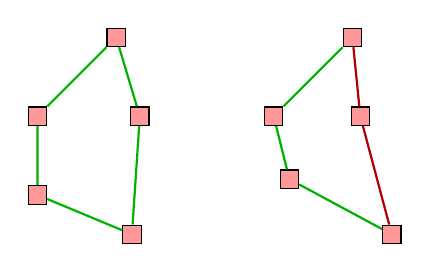
\begin{tikzpicture}[
	minimum width=0.2cm, 
	minimum height=0.2cm
	]
\node[draw, fill=red!40] at (0,2) (a1){}; 
\node[draw, fill=red!40] at (-1,1) (b1){}; 
\node[draw, fill=red!40] at (-1,-0) (c1){};
\node[draw, fill=red!40] at (0.2,-0.5) (d1){}; 
\node[draw, fill=red!40] at (0.3,1) (e1){}; 

\draw[thick, black!30!green] (a1) -- (b1) -- (c1) -- (d1) -- (e1) -- (a1);

\node[draw, fill=red!40] at (3,2) (a1){}; 
\node[draw, fill=red!40] at (2,1) (b1){}; 
\node[draw, fill=red!40] at (2.2,0.2) (c1){};
\node[draw, fill=red!40] at (3.5,-0.5) (d1){}; 
\node[draw, fill=red!40] at (3.1,1) (e1){}; 

\draw[thick, black!30!green] (a1) -- (b1) -- (c1) -- (d1);
\draw[thick, black!30!red] (d1) -- (e1) -- (a1);

 
\end{tikzpicture}
\captionof{figure}{Illustration af et succesfuldt (Venstre) og usuccesfuldt (Højre) afledningskast.}
\label{fig:afledning_tikz}
\end{Figure}

Der er ingen begrænsning for hvor mange købte afledningskast et hold kan kaste på en tur.




\end{multicols*}
\end{document}